\chapter{User Manual}

\section{Introduction}

The purpose of my program is to act as a skateboarding progress tracker and personal assistant. The program was built to aid skateboarding progress, maximise physical performance and enhance muscle memory by reminding the user of newly learnt tricks. The skateboard progress tracker also caters for the users skateboarding buying needs as it includes its very own skateboard part review hub. The integrated Google maps keeps a store of all of the skateparks and skate spots in the world, which skaters using the program can add to.

The intended audience of my program is currently purely for my client; however in the future, once a multi-user platform has been integrated the intended audience will be for the whole skating community.

As the skateboard progress tracker is still an uncompleted program, some of the functionality is not currently available in a graphical user interface format and not all of the validation is fully functional.

Currently, the version of the skateboard progress tracker includes a personalised profile tab where you can change the profile picture, email address and name to your own personal information. The tricks tab contains a table with a list of all the tricks in the database. You may delete tricks from your database by selecting the desired row and pressing delete. Another function on the tricks tab is the ability to add a trick to the database. With an easy to fill, side form that appears when 'add trick' is selected.This tab is used to keep a record of all the tricks that the user can do. The skatepark tab contains a customisable Google maps object which allows you to add and remove skateparks. This tab is used so that the user can plan on visiting new skateparks that they have never been to before. The review tab contains a table which displays all the reviews in the database. Functionality with the graphical user interface will be integrated in the next version of the program. The support tab allows the user to report any problems with the program, and request any additional functionality that they wish me to implement.





\section{Installation}

\textbf{System Requirements}

Before installing, your computer must meet the system requirements. As discussed in the analysis and design section (Subsections 1.7.1  and 2.3 respectively) I am developing this program for my client, therefore the system is built to run on:

\begin{itemize}
    \item 15.6" HD 1366x768 Screen
    \item i5-2450M Dual Core Processor (Sandy Bridge) 2.5GHz (overclocked to 3.1GHz) 3MB Cache
    \item 8GB DDR3 RAM
    \item 500GB HDD Memory
    \item Intel HD3000 Graphics Card
    \item Windows 7 Operating System
\end{itemize}

My program has been tested, and works on Windows 7 and Vista. Although the program hasn't been tested on Mac computers or windows 8, but the program should still work fine as long as the required programs are installed correctly as discussed below.




\subsection{Prerequisite Installation}

%include as many subsubsections as necessary for each piece of required software
\subsubsection{Installing Python 3.4}

\subsubsection{Installing PyQt}



\subsection{System Installation}

To install the system go to my personal github page and find the Comp4 repository (\url{http://www.github.com/BenKeppie}). Click on the download zip button and then save the file in an appropriate place on your hard drive.

\begin{figure}[H]
    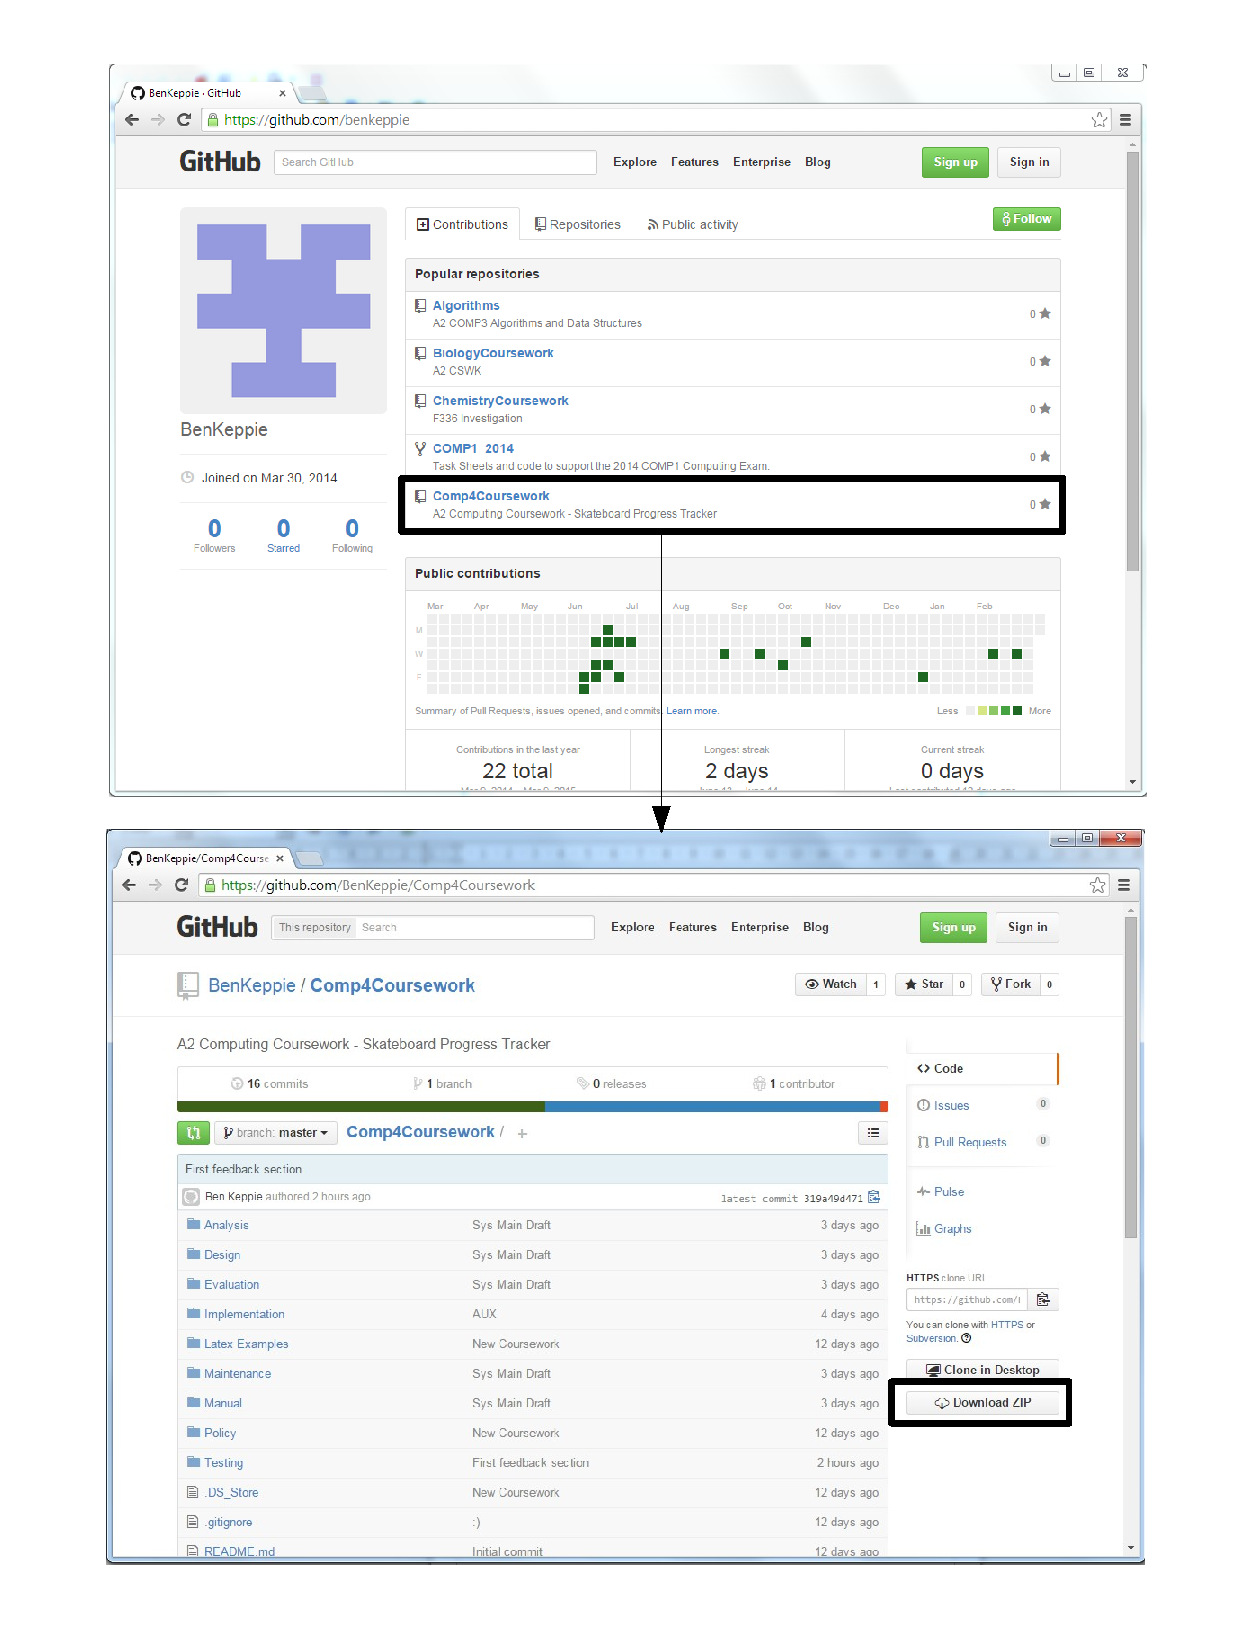
\includegraphics[width=\textwidth]{./Manual/Images/BenGithub.pdf}
    \caption{Downloading Skateboarding Progress Tracker Application} \label{fig:Downloading Program}
\end{figure}

To extract the files to a usable form you will need to extract the zip file. To do this you need to find the downloaded zip file, right click on it and save the extracted folder in an appropriate destination.

\begin{figure}[H]
    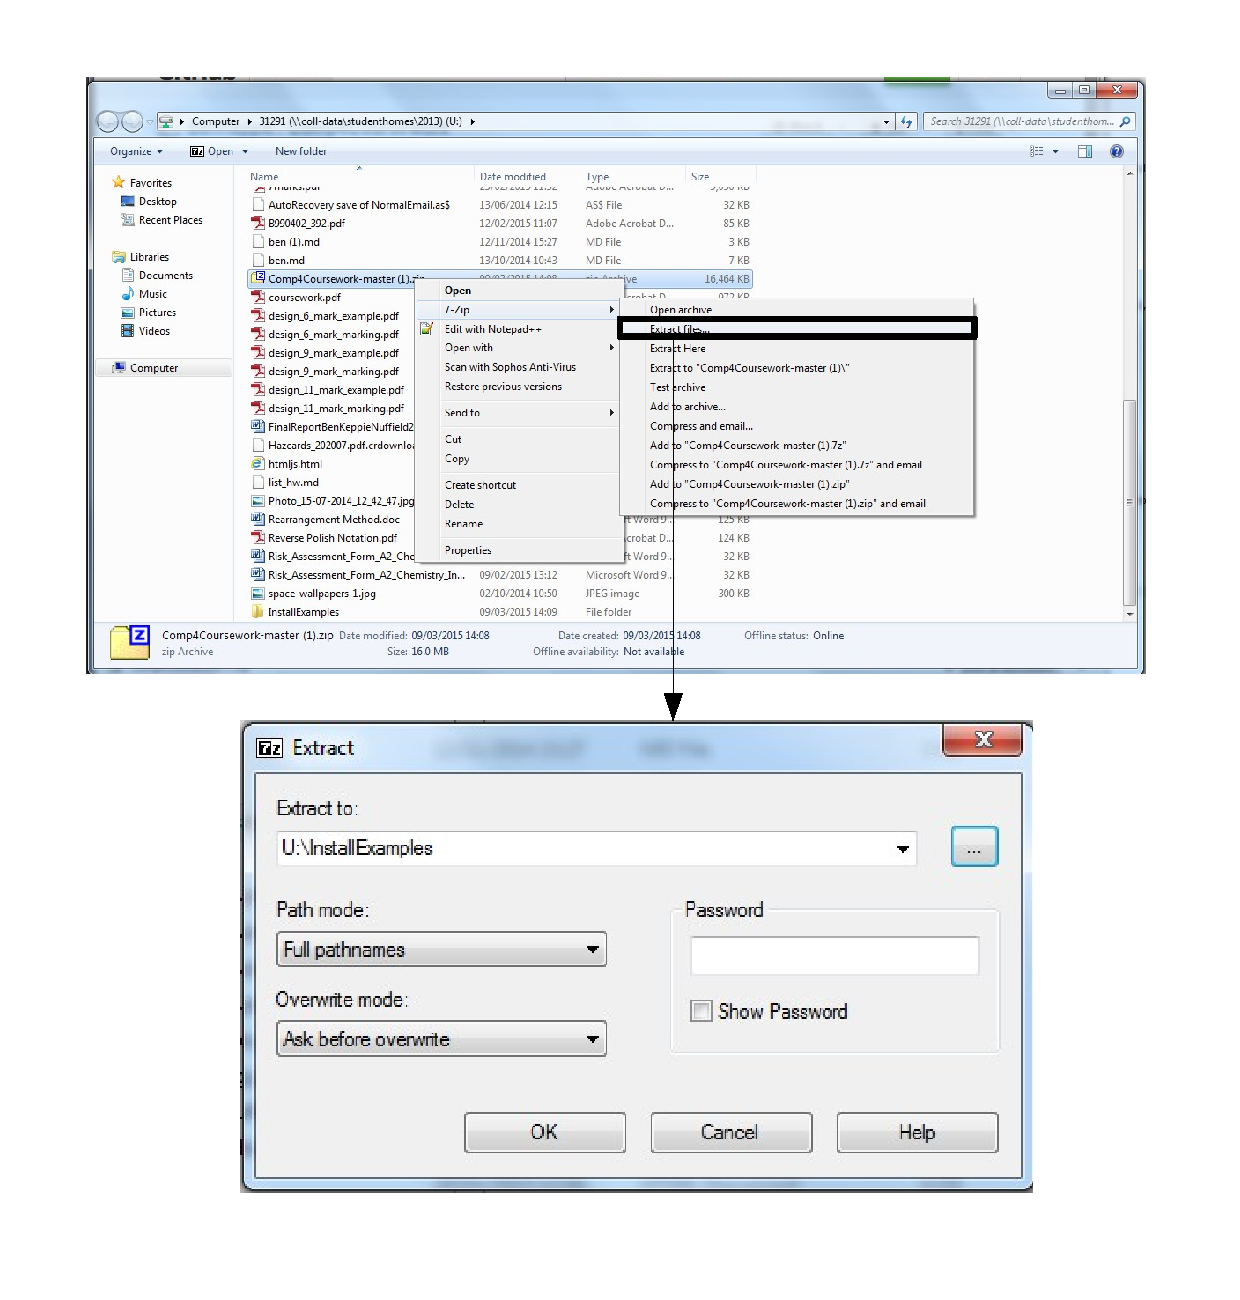
\includegraphics[width=\textwidth]{./Manual/Images/ExtractZIP.pdf}
    \caption{Extracting the zip File} \label{fig:Extracting ZIP}
\end{figure}

The system is now available to run as long as the appropriate programs discussed above are installed.


\subsection{Running the System}

To run the system, open the file location that you extracted the zip file to previously and navigate into the folder 'Implementation' and then click on the file 'main\_window.pyw', the program will now be loading, as shown by the start up of the splash screen.

\begin{figure}[H]
    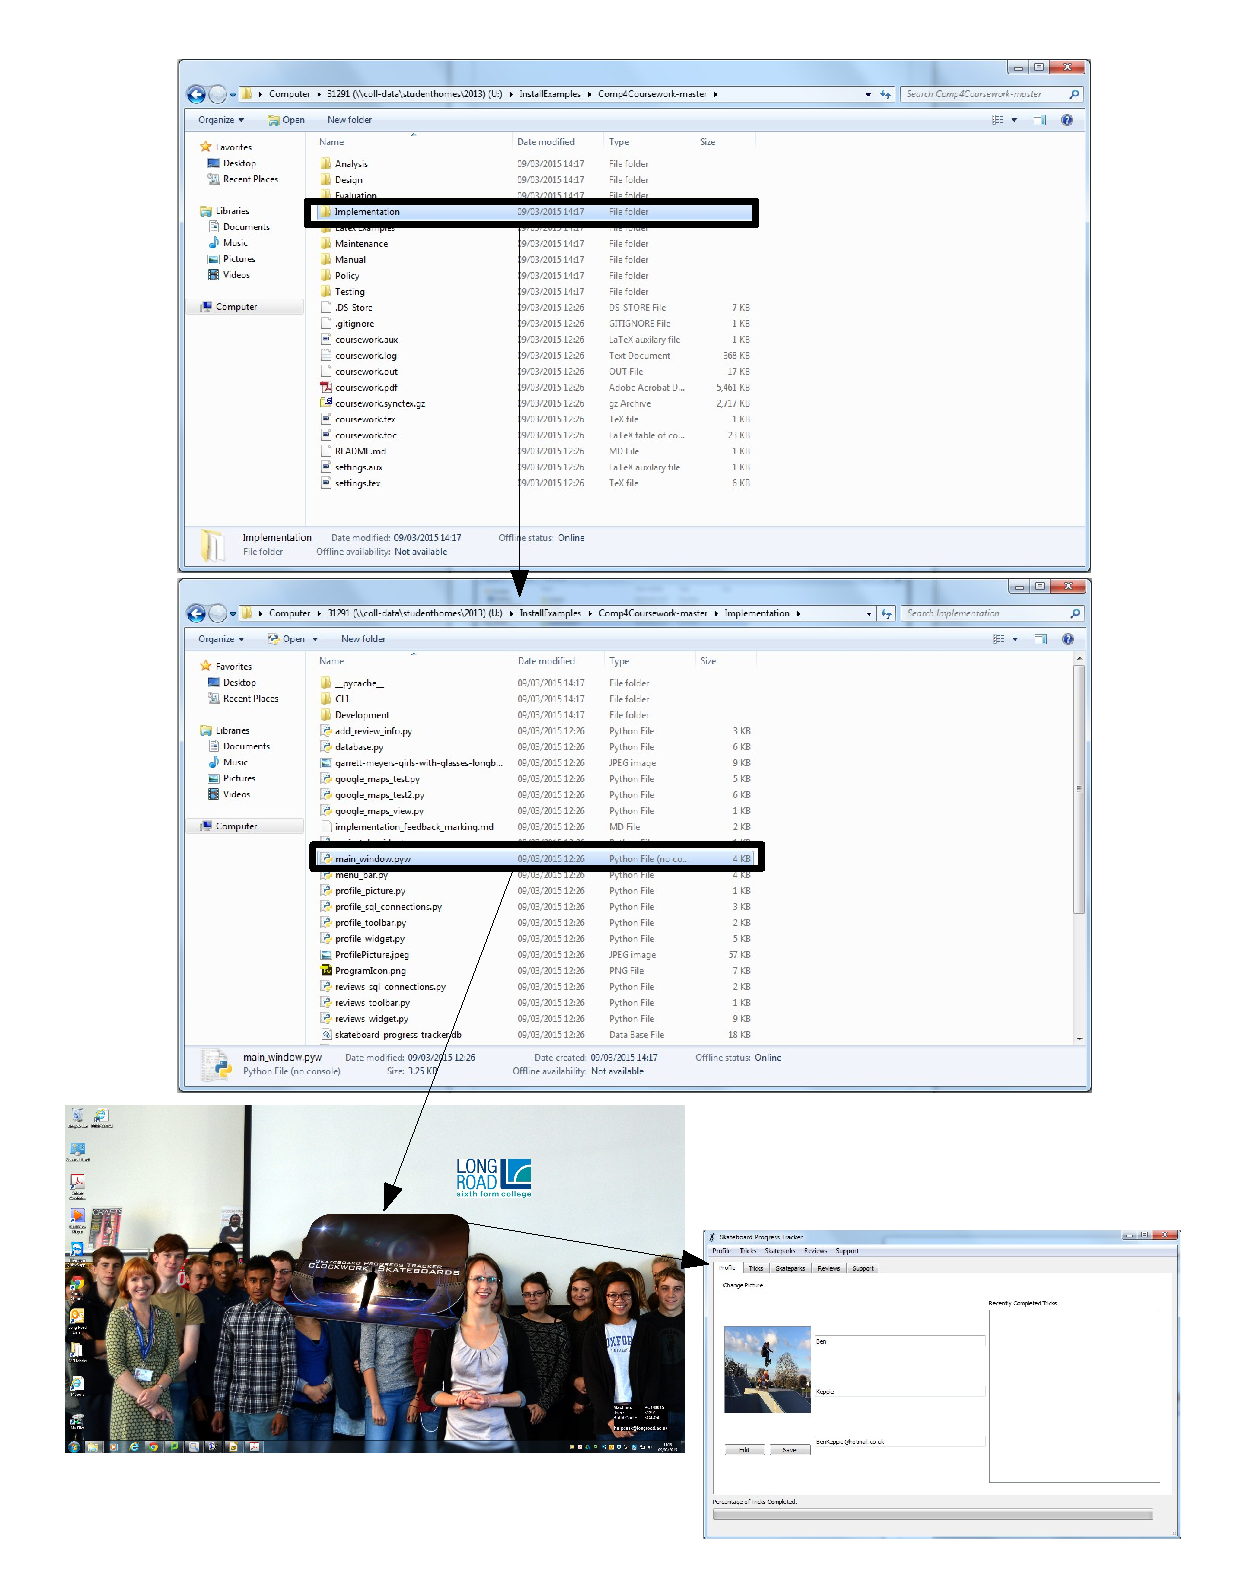
\includegraphics[width=\textwidth]{./Manual/Images/RunningProgram.pdf}
    \caption{Starting up the program} \label{fig:Running Program}
\end{figure}







\section{Tutorial}

\subsection{Introduction}

\subsection{Assumptions}

\subsection{Tutorial Questions}

%include as many subsubsections as necessary for each question in your list
\subsubsection{Question 1}

\subsubsection{Question 2}

\subsection{Saving}

My program saves information automatically due to the underlying SQL framework.

\subsection{Limitations}

As discussed in the introduction some sections are not fully implemented into a graphical user interface.

\section{Error Recovery}

%include as many subsections as necessary for each error
\subsection{Error 1}

\subsection{Error 2}






\section{System Recovery}

\subsection{Backing-up Data}

Save to an external hard drive/USB stick

\subsection{Restoring Data}

Copy the database file back.